\section{API}

A \textit{Web} API é composta por 2 módulos principais (API e Service) e um conjunto de módulos auxiliares. Enquanto que a API lida com pedidos e respostas HTTP e o \textit{Service} é responsável por implementar a lógica do sistema, existem ainda os repositórios (sendo que cada um se responsabiliza por implementar a sua própria lógica de acesso à base de dados) e o índice de imagens (responsável por tratar todas as operações associadas às mesmas).

\begin{figure}[h]
	\centering
	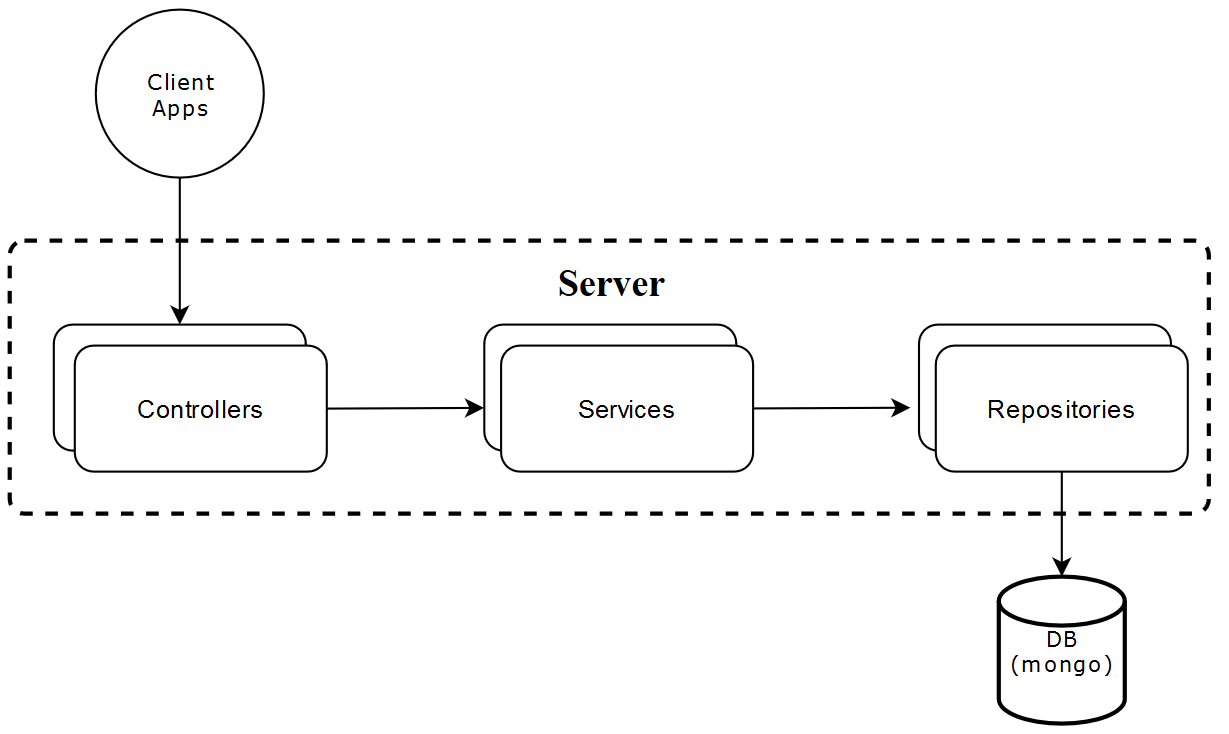
\includegraphics[scale=.50]{api_architeture}
	\caption{Diagrama de arquitetura da API}
\end{figure}

\subsection{API}
Este módulo é responsável por definir os endpoints e lidar com a receção e envio dos pedidos/respostas HTTP. Cada endpoint tem associada uma função que é executada que efetua à chamada ao serviço adequada para realizar a operação solicitada pelo utilizador. \par \medskip

Na próxima página, encontra-se a tabela das operações possíveis de efetuar na API. Refere-se também o método e o URL do pedido a efetuar. Estes pedidos encontram-se também definidos na wiki do projeto. \par \medskip

É de notar que todos os pedidos definidos têm o preâmbulo \textit{/api} e que os que começam por \textit{/auth} necessitam de autenticação prévia por parte do cliente da API. \par \medskip

\newpage

\begin{figure}[h]
	\centering
	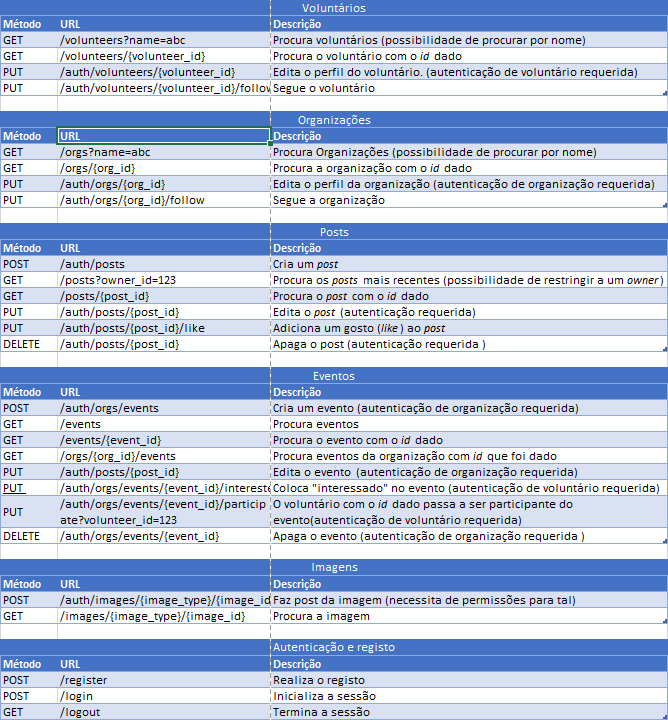
\includegraphics[scale=.70]{endpoints_table}
	\caption{Lista de \textit{endpoints}}
\end{figure}

Para além das funções já referidas, são também definidos (e utilizados) \textit{middlewares} nesta camada de maneira a garantir o cumprimento da necessidade de autenticação aquando de certas operações. \medskip

\newpage

\subsection{Serviço}
(todo service)

\subsection{Repositórios e acesso a base de dados}
(todo repositories and base repository)

\subsection{Base de Dados}

\subsection{Autenticação}

\subsection{Imagens}
(todo pictures)

\subsection{Documentação e definição da API}